\documentclass{article}
\usepackage{graphicx} % Required for inserting images
\usepackage{amssymb}

\title{Multiple data sources model time model}
\author{Johnny Kelsey }

\date{August 2025}

\begin{document}

\maketitle

\section{Multiple data sources model}

How could we model the time taken by a business team having to check internal and external data sources for an address?

Let's assume there are $N$ internal data sources, and $M$ external data sources.

The time taken to check these sources varies.

A stochastic process model is a potentially useful way to model the time taken to check addresses. This approach recognises that the time taken for each check is not a fixed quantity, but is a random variable, which better reflects real-world variability.

\section{Building the model}

First, we need to define the variables for each type of data source.

\begin{itemize}
    \item $T_{int}$: The random variable representing the time taken to check a single internal data source.
    \item $T_{ext}$: The random variable representing the time taken to check a single external data source.
    \item $N$: The number of internal data sources (constant).
    \item $M$: The number of external data sources (constant).
    \item $X$: The total time taken to find a valid address.
\end{itemize}

We assume that the time taken to check each source is an \emph{independent and identically distributed} (i.i.d.) random variable. This means the time to check one source has no effect on the time to check a different data source.

The process of checking for an address is sequential - a team member can only check a single data source at a time. A team member checks a source, and if the address is found and verified, the process stops. Otherwise, they move to the next source.

We assume the team member checks internal sources first, followed by external sources.

The total time, $X$, is the sum of the times taken to check each source until the address is found.

We have

\begin{equation}
X = \sum_{i=1}^{k} T_{i]}
\end{equation}
where $k$ is the number of sources checked and $T_{i}$ is the time taken for the $i$-th source. Here, $k$ is also a random variable, since we are assuming that the address could be found in any of the data sources.

We model the time taken for each data source check using a probability distribution. An appropriate distribution for this context would be the \emph{exponential distribution}. This is the probability distribution of the distance between events, commonly used to model a process in which events occur continuously and independently, at a constant average rate.

We say that the time to check an internal source, $T_{int}$,  follows an exponential distribution with rate $\lambda_{int}$. The average time to check an internal source is $\frac{1}{\lambda_{int}}$.

Similarly, we assume that the time to check an external source, $T_{ext}$, follows an exponential distribution with rate $\lambda_{ext}$. The average time to check an external source is $\frac{1}{\lambda_{ext}}$.

We also introduce probabilities for success at each data source:

\begin{itemize}
\item $p_{int}$: The probability of finding the correct address in any single internal source.
\item $p_{ext}$: The probability of finding the correct address in any single external source.
\end{itemize}

Recall that we assume the process is the following: the team member checks internal sources first, one by one. If they fail to find a good address after checking all $N$ internal sources, they move on to the $M$ external sources.

The total time X can be broken down into two components:

\begin{itemize}
\item Time spent on internal sources: The time taken to check internal sources until a good address is found, or all $N$ sources have been checked.

\item Time spent on external sources: The time taken to check external sources, but only if no good address was found in the internal sources.
\end{itemize}

\subsection{Calculating the expected total time}

While the total time $X$ is a random variable, we can calculate its expected value, $\mathbb{E}[X]$, which is the average time a team member would spend on this task. The expected time is the sum of the expected times for each step, weighted by the probability of reaching that step.

A fairly simple approach is to think in terms of the probability of success at each stage.

We have:

\begin{itemize}
    \item Probability of success at source 1: $p_{int}$. 
    \item Expected time: $p_{int} \times \mathbb{E}[T_{int}]$.
    \item Probability of success at source 2: $(1 - p_{int}) \times p_{int}$. 
    \item Expected time: $(1 - p_{int}) \times p_{int} \times 2 \times \mathbb{E}[T_{int}]$.  
    \item ... and so on ...
\end{itemize}

We can simplify and use a more direct approach by considering the states.

\begin{itemize}
    \item Let $P_{Ifail}$ be the probability of failing to find the address in all $N$ internal data stores. Then we have $\left( 1 - p_{int} \right)^{N}$.
    \item Let $\mathbb{E}\left[T_{Itotal} \right]$ be the expected time spent checking all of the internal data sources,
     \item Let $\mathbb{E}\left[T_{Etotal} \right]$ be the expected time spent checking all of the external data sources.
\end{itemize}

Let's work through the logic.

\subsection{Checking internal data sources}

We would like to find a formal way of describing the process of finding a valid address, which is the sum of the time spent checking each internal source, weighted by the probability of the search ending at that source.

This is how we describe the events in the process:

\begin{itemize}
    \item $T_{int}$: The random variable representing the time to check a single internal source.
    \item $\mathbb{E}\left[ T_{int} \right]$: The expected time taken to check a single internal data source.
    \item $p_{int}$: The probability of finding a good address in any single internal data source.
    \item $N$: the total number of internal data sources.
\end{itemize}

The search process is sequential; it stops as soon as a valid address is found.

\begin{itemize}
    \item Case 1: Success at the 1st internal source.
    \begin{itemize}
        \item Probability: $p_{int}$.
        \item Time spent: $T_{int}$.
        \item Expected time spent: $p_{int} \times \mathbb{E}\left[T_{int}\right]$ 
    \end{itemize}
    \item Case 2: Failure at the 1st source, but success at the 2nd.
    \begin{itemize}
        \item Probability: $\left(1 - p_{int} \right) \times p_{int}$.
        \item Time spent: $2 \times T_{int}$.
        \item Expected time spent: $\left(1 - p_{int}\right) \times p_{int} \times 2 \times \mathbb{E}\left[T_{int}\right]$
    \end{itemize}
    \item Case 3: Failure at the 2nd source, but success at the 3rd.
    \begin{itemize}
        \item Probability: $\left(1 - p_{int} \right)^{2} \times p_{int}$.
        \item Time spent: $3 \times T_{int}$.
        \item Expected time spent: $\left(1 - p_{int}\right)^{2} \times p_{int} \times 3 \times \mathbb{E}\left[T_{int}\right]$
    \end{itemize}
\end{itemize}
This pattern continues for all of our $N$ internal data sources. The total expected time for the internal search is the sum of the expected times for all possible successful outcomes.

Putting this all together into an equation for the expected time taken for each outcome, we have:

\begin{equation}
   \mathbb{E}\left[T_{Totalint}\right] = \sum_{i=1}^{N} \left(1 - p_{int} \right)^{i-1} \times p_{int} \times i \times \mathbb{E}\left[ T_{int}\right]
\end{equation}
This equation represents the sum of the probabilities of finding the address at each specific source, multiplied by the time it would take to reach that source.

\subsection{Checking external data sources}

We assume that the team member has exhausted all the internal data sources - the address might be missing, or it might be incomplete, or they might be trying to verify or validate the data.

The key insight is that a team member only starts checking external sources \emph{if and only if} they fail to find a valid address in all of the internal sources. This makes the time spent on external sources a conditional event.

\begin{itemize}
    \item $P_{Ifail}$ is the probability that the internal search fails. This is the probability of the first internal data source failing, and the second failing, ..., and the $N$-th source failing.
    \item So we have $P_{Ifail} = \left(1 - p_{int}\right)^{N}$
\end{itemize}
So the expected total time spent on internal sources. $\mathbb{E}[T_{Etotal}]$, can be expressed informally as 

\begin{equation}
  \mathbb{E}[T_{Etotal}] = P_{Ifail} \times \mathbb{E}[P_{Text} | P_{Ifail}] 
\end{equation}


where $P_{Ifail}$ is the probability of being unable to confirm the data using internal sources, and $P_{Text}$ is the probability of a certain time taken to locate the address in external sources. So we have a conditional expectation, such that the total expected value of an event is the probability of its condition occurring, multiplied by the expected value of the event given that condition. Note that we have $\mathbb{E}[P_{Text} | P_{Ifail}]$, which is the expected time to find an address among the external data sources, given that all internal sources have been exhaustively checked, and failed to find the address. The model assumes that the internal and external searches are independent processes, so this simply becomes the expected time of the external search process itself.

Breaking this down further, the expected time taken to find an address in a sequence of $M$ external sources is the sum of the expected times for each of the possible outcomes. Let $T_{j}$ be the time taken for the $j$-th external source.

\begin{itemize}
    \item Case 1: Success at 1st external source.
    \begin{itemize}
        \item Probability: $p_{ext}$
        \item Time: $1 \times \mathbb{E}\left[T_{ext}\right]$.
    \end{itemize}
    \item Case 2: Success at 2nd external source.
    \begin{itemize}
        \item Probability: $\left(1 - p_{ext}\right) \times p_{ext}$.
        \item Time: $2 \times \mathbb{E}\left[T_{ext}\right]$.
    \end{itemize}
    \item $\cdots$
    \item Case $M$: Success at the $M$-th external source.
    \begin{itemize}
        \item Probability: $\left(1 - p_{ext}\right)^{M-1} \times p_{ext}$
        \item $M \times \mathbb{E}\left[T_{ext}\right]$
    \end{itemize}
    \item Case $M+1$: Failure to find the address after checking all $M$ sources.
    \begin{itemize}
        \item Probability: $\left(1 - p_{ext}\right)^{M}$.
        \item Time: $M \times \mathbb{E}\left[ T_{ext} \right]$
    \end{itemize}
\end{itemize}
So the total expected time is the sum of the expected time for each of the above cases:

\begin{equation}
    \mathbb{E}\left[Text \right] = \sum_{j=1}^M \left(1 - p_{ext}\right)^{j-1} \times p_{ext} \times j \times \mathbb{E}\left[ T_{ext} \right] + \left(1 - p_{ext} \right)^{M} \times M \times \mathbb{E}\left[ T_{ext}\right] 
\end{equation}
This formula is the standard way to calculate the expected number of trials in a limited geometric distribution (recall that we have a finite number of data sources), We get those probabilities and multiply them by the expected time per trial.

\section{Simulation}

The model above can be translated into code, and used to simulate the process of an individual team member looking for an address over a number of different trial runs.

%\begin{figure}
%    \centering
%    \includegraphics[width=0.5\linewidth]{address_search_time_distribution.png}
%    \caption{Model: expected time taken checking multiple data sources.}
%    \label{fig:placeholder}
%\end{figure}

\begin{figure}
    \centering
    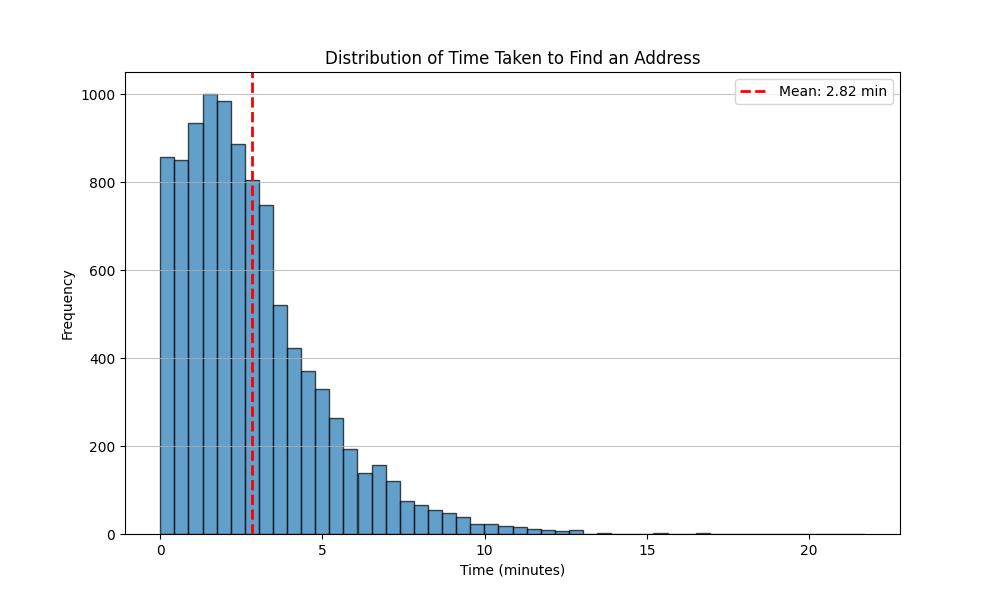
\includegraphics[width=1\linewidth]{distribution1.jpg}
    \caption{Time taken to check multiple data sources.}
    \label{fig:modelrun1}
\end{figure}
The code allows us to see the results of running the model given different parameters. In order to run the code, we need to define a few parameters. We define the following:

\begin{itemize}
    \item number of internal data sources: 3
    \item number of external data sources: 5
    \item $p_{int}$: the probability of finding the correct address in any single internal source: 0.1.
    \item $p_{ext}$: the probability of finding the correct address in any single external source: 0.1.
    \item average time taken to check internal data sources: 0.5 (minutes).
    \item average time taken to check external data sources: 2.82 (minutes).
\end{itemize}

The model was run for $10000$ trials. Figure (\ref{fig:modelrun1}) shows the results.  

\end{document}
